\section{Beispiele}

Neben der Zeitkomplexität $T(n)$ werden wir uns nun auch mit der Speicherkomplexität $S(n)$ beschäftigen.

\begin{*anmerkung}
	Es nicht unbedingt entscheidend, alle Komplexitäten auswendig zu lernen. Vielmehr sollte man wissen, wie die Algorithmen dahinter arbeiten und sich so die Komplexitäten herleiten.
\end{*anmerkung}

\subsection{Fakultät}
\begin{lstlisting}
recursive function fac (n) result (res) 
 integer :: n
 integer :: res
 
 if (n == 1) then 
  res = 1
 else
  res = n*fac(n-1)
 end if
end function fac
\end{lstlisting}
$\Rightarrow T(n) = \Theta(n)$, $S(n)=\Theta(n)$

\begin{lstlisting}
function fac_iterativ (n)
 integer :: n, fac_iterativ, i
 
 fac_iterativ = 1
 
 do i = 1, n
  fac_iterativ = fac_iterativ * i
 end do
end function fac_iterativ
\end{lstlisting}
$\Rightarrow T(n)=\Theta(n)$, $S(n)=\Theta(1)$

\subsection{Reverse String}
\begin{lstlisting}
recursive function reverse (string) result (res)
 character (*), intent (in) :: string
 character (len (string)) :: res

 if (len (string) == 0) then
  res = ""
 else
  res = string(len(string):)//reverse(string(:len(string)-1))
 end if
end function reverse
\end{lstlisting}
$\Rightarrow T(n) = \Theta(n)$, $S(n)=\Theta(n)$

\begin{lstlisting}
program reverse_iterativ
 character(80) :: str = "This is a string"
 character :: temp
 integer :: i, length

 write(*,*) str
 length = len_trim(str) 
 ! Ignores trailing blanks. 
 ! Use len(str) to reverse those as well
 
 do i = 1, length/2
  temp = str(i:i)
  str(i:i) = str(length+1-i:length+1-i)
  str(length+1-i:length+1-i) = temp
 end do
 
 write(*,*) str
end program reverse_iterativ
\end{lstlisting}
$\Rightarrow T(n) = \Theta(n)$, $S(n)=\Theta(n)$

\subsection{Primzahl}

Um zu überprüfen, ob eine Zahl eine Primzahl ist, muss man immer bis zur Wurzel dieser Zahl auf Teiler prüfen. Egal ob man das rekursiv oder iterativ macht, $T(n)=\mathcal{O}(\sqrt{n})$. Die Speicherkomplexität ist beim rekursiven schwer vorher zu sagen, beim iterativen Algorithmus ist die $S(n)=\Theta(1)$.

\subsection{\person{Fibinacci}-Zahlen}
\begin{lstlisting}
recursive function fibR(n) result(fib)
 integer, intent(in) :: n
 integer :: fib

 select case (n)
  case (:0); fib = 0
  case (1); fib = 1
  case default; fib = fibR(n-1) + fibR(n-2)
 end select
end function fibR
\end{lstlisting}
$\Rightarrow T(n) = \Theta(\Phi^n)$, $S(n)=\mathcal{O}(2^n)$

\begin{lstlisting}
function fibI(n)
 integer, intent(in) :: n
 integer, parameter :: fib0 = 0, fib1 = 1
 integer :: fibI, back1, back2, i

 select case (n)
  case (:0); fibI = fib0
  case (1); fibI = fib1
  case default
   fibI = fib1
   back1 = fib0
   do i = 2, n
    back2 = back1
    back1 = fibI
    fibI   = back1 + back2
   end do
 end select
end function fibI
\end{lstlisting}
$\Rightarrow T(n) = \Theta(n)$, $S(n)=\Theta(1)$

Man kann die $n$-te \person{Fibonacci}-Zahl $F_n$ auch direkt berechnen:
\begin{align}
	F_n = \frac{\Phi^n-(1-\Phi^n)}{\sqrt{5}}\notag
\end{align}
Hier wird eine ganzzahlige Potenzierung benötigt, die eine Komplexität von $T(n)=\Theta(\log_2 n)$ hat.

\subsection{Ganzzahliges Potenzieren}

Wenn man naiv vorgeht, ist Potenzieren nichts anderes als Multiplikation $n$ mal mit sich selbst. Dann sind die Komplexitäten: $T(n)=\Theta(n)$, $S_{iter}(n)=\Theta(1)$ und $S_{rek}(n)=\Theta(n)$.

Man kann den Prozess aber noch deutlich verbessern. Soll man zum Beispiel $5^{10}=5^8\cdot 5^2$ berechnen, so berechnet man $5^2=25$, $5^4=5^2\cdot 5^2=625$, $5^8=5^4\cdot 5^4=390.625$ und abschließend $5^{10}=5^2\cdot 5^8=9.765.625$.
\begin{itemize}
	\item rekursiv: $T(n)=\Theta(\log_2 n)$, $S(n)=\Theta(\log_2 n)$
	\item iterativ: $T(n)=\Theta(\log_2 n)$, $S(n)=\Theta(1)$
\end{itemize}

Man kann das Potenzieren auch direkter machen: $x^n=e^{\ln x^n}=e^{n\cdot\ln x}$. Allerdings braucht man hier die Funktionen $e^x$ und $\ln$, die insgesamt langsamer als die iterative Methode sind.

\subsection{Größter gemeinsamer Teiler}
Es gilt:
\begin{align}
	\ggT(a,b) &= \ggT(a-b,b) = \ggT(a-2b,b) = ... \notag \\
	&= \ggT(a\text{ mod } b,b) = \ggT(b, a\text{ mod } b) \notag
\end{align}

\begin{proposition}[von Lamé]
	$\forall k\ge 1,k\in\natur$, wenn $a>b\ge 0$ und $b<F_{k+1}$ gilt, dann macht $\ggT(a,b)$ höchstens $k-1$ rekursive Aufrufe. Zwei aufeinanderfolgende \person{Fibonacci}-Zahlen sind der worst case für den euklidischen Algorithmus:
	\begin{align}
		\ggT(F_{k+1},F_k) = \ggT(F_k,F_{k+1}\text{ mod } F_k) = \ggT(F_k,F_{k-1})\notag
	\end{align}
\end{proposition}
Da $F_k=\frac{\Phi^n}{\sqrt{5}}$ mit $\Phi=\frac{1+\sqrt{5}}{2}$ folgt
\begin{itemize}
	\item rekursiv: $T(n)=\mathcal{O}(\log_\Phi\min\{a,b\})$
	\item iterativ: $T(n)=\mathcal{O}(\log_\Phi\min\{a,b\})$
\end{itemize}

\subsection{Binominialkoeffizient}

Der Binominialkoeffizient lässt sich rekursiv wie folgt berechnen:
\begin{align}
	\binom{n}{k} = \binom{n-1}{k-1}+\binom{n-1}{k}\notag
\end{align}
$\Rightarrow T(n)=\mathcal{O}(2^n)$, $S(n)=\mathcal{O}(n)$

Der Algorithmus klappt auch iterativ, deshalb $T(n)=\mathcal{O}(n^2)$, $S(n)=\Theta(n)$

Man kann den Binominialkoeffizienten auch ganz normal ausrechnen:
\begin{align}
	\binom{n}{k}=\frac{n}{1}\cdot\frac{n-1}{2}\cdot\frac{n-2}{3}\cdot\dots\cdot\frac{n-k+1}{k}\notag
\end{align}
$\Rightarrow T(n)=\Theta(k)=\mathcal{O}(n)$, $S(n)=\Theta(1)$

\subsection{Collatz-Funktion}

Lothar Collatz hat 1937 eine interessante Rechenvorschrift für Zahlen entwickelt, deren Problem bis heute noch nicht gelöst wurde.

\begin{lstlisting}
collatzFun(p,n)
 do while (n /= 1)
  if(mod(n,2) == 1) then
   n=p*n+1
  else
   n = n/2
  end if
 end do
end collatzFun
\end{lstlisting}

Für $p=5$ ergibt sich:
\begin{center}
	\begin{tabular}{l|p{7cm}}
		\rowcolor{lightgray} \textbf{$n$} & \texttt{collatzFun(5,n)} \\
		\hline
		1 & 1 \\
		2 & $2\to 1$ \\
		3 & $16\to 8\to 4\to 2\to 1$ \\
		4 & $4\to 2\to 1$ \\
		5 & $26\to 13\to 66\to 33\to 166\to 83\to 416\to 208\to 104\to 52\to 26\to\dots$
	\end{tabular}
\end{center}
$\Rightarrow$ nicht immer berechenbar, das heißt, die Funktion kommt nie zum Ende

Für $p=3$ (originales Collatz-Problem) ergibt sich:
\begin{center}
	\begin{tabular}{l|p{7cm}}
		\rowcolor{lightgray} \textbf{$n$} & \texttt{collatzFun(3,n)} \\
		\hline
		1 & 1 \\
		2 & $2\to 1$ \\
		3 & $10\to 5\to 16\to 8\to 4\to 2\to 1$ \\
		4 & $4\to 2\to 1$ \\
		5 & $16\to 8\to 4\to 2\to 1$
	\end{tabular}
\end{center}

Es stellt sich die Frage, ob dieses Problem immer berechenbar ist. Man hat gezeigt, dass es für $p=3$ bis zu $n<2^{61}$ berechenbar ist.

\subsection{Multiplikation zweier $n$-stelliger Zahlen $x$ und $y$}

Bei einer iterativen Multiplikation, so wie man sie schriftlich gelernt hat, beträgt die Komplexität $T(n)=\Theta(n^2)$ oder eben auch allgemein $T(x\cdot y)=\Theta(\log_b x\cdot\log_b y)=\Theta(m\cdot n)$ mit $m=\text{digits($x$)}$ und $n=\text{digits($y$)}$.

Falls man bis jetzt die Vermutung hatte, dass rekursive Algorithmen immer schlechter als iterative Algorithmen sind, hier ist ein Gegenbeispiel: Wenn man die Zifferngruppen rekursiv halbiert ergibt sich eine Komplexität von $T(n)=\Theta(n^{\log_2 3})=\Theta(n^{1,525})$.

Der \person{Schönhage-Strassen}-Algorithmus, eine diskrete Fourier-Transformation, war von 1971 bis 2007 (in der Vorlesung war es auch nicht aktueller) der schnellste Multiplikationsalgorithmus mit einer Komplexität von $T(n)=\Theta(n\cdot\log n\cdot\log\log n)$.

\subsection{Matrizenmultiplikation}

Die iterative Methode hat eine Komplexität von $T(n)=\Theta(n^3)$. Das ist die Methode, die auch in der Schule/im Studium gelehrt wird.

Auch hier ist die rekursive Variante wieder etwas schneller, \person{Strassen} fand einen Algorithmus mit einer Komplexität von $T(n)=\Theta(n^{\log_2 7})=\Theta(n^{2,8075})$.

Der beste bis heute bekannte Algorithmus setzt auf eine Vermischung von iterativen und rekursiven Funktionen und hat eine Komplexität von $T(n)=\mathcal{O}(n^{2,376})$.

\subsection{Zyklische Zahl}

Finde Ziffern $z_1,...,z_n$ mit:
\begin{align}
	5\cdot[z_1z_2...z_n]_{10}=[5z_1z_2...z_n]_{10}\notag
\end{align}

Ein einfaches Durchprobieren aller Zahlen bis zu einer Zahl $n$ erzeugt einen Aufwand von $T(n)=\mathcal{O}(n\log n)$. Mit systematischer Berechnung der Ziffern von hinten nach vorne beträgt der Aufwand nur noch $T(n)=\mathcal{O}(\log_2 n)$, wenn $n$ die gesuchte Zahl ist.

Die gesuchte Zahl ist übrigens $n=10.204.081.632.653.061.224.489.795.918.367.346.938.775$. \\
Als Wort: "'10 Sextilliarden 204 Sextillionen 81 Quintilliarden 632 Quintillionen 653 Quadrilliarden 61 Quadrillionen 224 Trilliarden 489 Trillionen 795 Billiarden 918 Billionen 367 Milliarden 346 Millionen 938 Tausend 775"' \smiley{}.

\subsection{Türme von Hanoi}

\begin{center}
	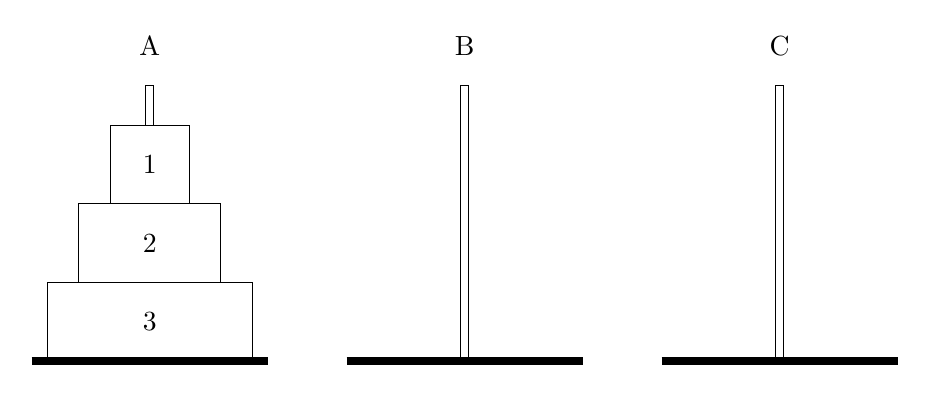
\begin{tikzpicture}
	\draw[line width=1mm] (0,0) -- (3,0);
	\draw[line width=1mm] (4,0) -- (7,0);
	\draw[line width=1mm] (8,0) -- (11,0);
	
	\draw (0.2,0) rectangle (2.8,1);
	\draw (0.6,1) rectangle (2.4,2);
	\draw (1.0,2) rectangle (2.0,3);
	\node at (1.5,2.5) (1) {1};
	\node at (1.5,1.5) (2) {2};
	\node at (1.5,0.5) (3) {3};
	
	\draw (1.45,3) rectangle (1.55,3.5);
	\draw (5.45,0) rectangle (5.55,3.5);
	\draw (9.45,0) rectangle (9.55,3.5);
	
	\node at (1.5,4) (A) {A};
	\node at (5.5,4) (B) {B};
	\node at (9.5,4) (C) {C};
	\end{tikzpicture}
\end{center}

Dieses Problem lässt sich nur rekursiv rechnen. Der Aufwand dafür beträgt $T(n)=2^n-1$.

\begin{center}
	\begin{longtable}{p{1cm}|p{2cm}|p{2cm}|p{2cm}|p{2cm}}
		\rowcolor{lightgray}
		& \textbf{Schritt} $i$ & \textbf{Scheibe} $d$ & \textbf{Quelle} $s$ & \textbf{Ziel} $t$ \\
		\hline
		$n=1$ & 1 & 1 & A & C \\
		\hline\hline
		$n=2$ & 1 & 1 & A & B \\
		\hline
		 & 2 & 2 & A & C \\
		 \hline
		 & 3 & 1 & B & C \\
		 \hline\hline
		 $n=3$ & 1 & 1 & A & C \\
		 \hline
		  & 2 & 2 & A & B \\
		  \hline
		  & 3 & 1 & C & B \\
		  \hline
		  & 4 & 3 & A & C \\
		  \hline
		  & 5 & 1 & B & A \\
		  \hline
		  & 6 & 2 & B & C \\
		  \hline
		  & 7 & 1 & A & C
	\end{longtable}
\end{center}

Im $i$-ten Schritt finden dann folgende Schritt statt:
\begin{itemize}
	\item Scheibe $k$ wird bewegt, mit \texttt{mod(i,2**(k-1))} = 0, aber \texttt{mod(i,2**k) != 0}
	\item Scheibe $k$ wird zum ersten Mal im Schritt $2^{k-1}$ und dann alle $2^k$ Schritte bewegt
	\item Die größte Scheibe $n$ wird immer genau einmal im Schritt $2^{n-1}$ von A nach C bewegt, das heißt rückwärts durch die Positionsindizes, die nächstkleinere Scheibe $n-1$ zweimal vorwärts A $\to$ B $\to$ C, die nächstkleinere $n-2$ viermal rückwärts A $\to$ C $\to$ B $\to$ A $\to$ C, ...
\end{itemize}

\begin{*anmerkung}
	Der Legende nach soll die Welt zu dem Zeitpunkt untergehen, wenn dieses Problem mit $n=64$ Scheiben von einem Menschen gelöst wurde.
	
	Dafür benutzt man stattdessen einen Computer und das Programm von Unicomp, Inc (\url{https://www.fortran.com/F/ex_hanoi.html}, auch in meinen Github-Repository: \url{https://github.com/henrydatei/TU_PROG/blob/master/Tuerme_von_Hanoi.f95}).
	
	Dieses Programm wird bei $n=64$ einen Output von einem Zetabyte produzieren, was in etwa dem Internettraffic der Menschheit eines Jahres entspricht. Weiterhin würde mein Rechner rund 3,3 Millionen Jahre brauchen. Es dauert also noch ein bisschen bis zum Weltuntergang \smiley{}.
\end{*anmerkung}

\subsection{Kochkurve}

\begin{center}
	\begin{tikzpicture}[decoration=Koch snowflake, scale=0.8]
		\draw decorate{(0,0) -- ++(60:3)  -- ++(300:3) -- ++(180:3)};
		\draw decorate{ decorate{(4,0) -- ++(60:3)  -- ++(300:3) -- ++(180:3)}};
		\draw decorate{ decorate{ decorate{(8,0) -- ++(60:3)  -- ++(300:3) -- ++(180:3)}}};
		\draw decorate{ decorate{ decorate{ decorate{(12,0) -- ++(60:3)  -- ++(300:3) -- ++(180:3)}}}};
	\end{tikzpicture}
\end{center}

Die Komplexitäten lauten
\begin{itemize}
	\item rekursiv: $T(n)=\mathcal{O}(4^n)$
	\item iterativ: Algorithmus ist sehr kompliziert
\end{itemize}

\subsection{$n$-Damen-Problem}

Beim $n$-Damen-Problem geht es darum, $n$ Damen auf einen $n\times n$-Schachbrett zu verteilen, sodass keine Dame eine andere schlagen kann. Eine Dame kann alle Damen schlagen, die horizontal, vertikal oder diagonal zu ihr stehen.

Für $n=1$ gibt es genau 1 triviale Lösung, $n=2$ und $n=3$ haben keine Lösungen, für $n=4$ gibt es bis auf Symmetrien auch nur eine Lösung:
\begin{center}
	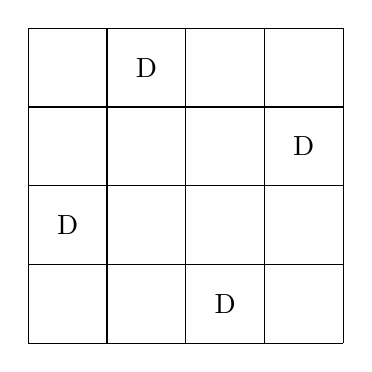
\begin{tikzpicture}
		\draw[step=1] (0,0) grid (4,4);
		\node at (0.5,1.5) (a) {D};
		\node at (1.5,3.5) (b) {D};
		\node at (2.5,0.5) (c) {D};
		\node at (3.5,2.5) (d) {D};
	\end{tikzpicture}
\end{center}

Will man alle Lösungen finden kann man die $n$ Damen beliebig auf die $n^2$ Felder verteilen. Dann muss man $\binom{n^2}{n}$ Möglichkeiten durchprobieren. Verteilt man nur auf jeder Spalte eine Dame, so hat man noch $n^n$ Möglichkeiten. Bei zusätzlich nur noch einer Dame pro Zeile sind es nur noch $n!$ Möglichkeiten. Wenn auch Diagonalen berücksichtigt werden sollen, gibt es viel weniger Möglichkeiten. Da eine
systematische Planung vorausschauend alle bedrohten Felder für weitere Platzierungen kennen müsste, wird zur Lösung \begriff{Backtracking} verwendet.

\subsection{Legepuzzle}

Eine Legepuzzle ist ein zweidimensionales Puzzle mit $n$ Teilen.

Löst man dieses Puzzle rekursiv naiv, also vergleicht eine Seite eines Teils mit jeweils allen offenen Stellen, so hat man $T(n)=\mathcal{O}(n^2)$. Löst man dies iterativ mit $k$ Teilengen, zum Beispiel Farbgruppen mit $\approx\frac{n}{k}$ Teilen, wobei $k\le\frac{n}{k}$, also zum Beispiel $k=\sqrt{n}=\frac{n}{k}$: $T_k(n)=\mathcal{O}(n+\frac{n^2}{k}+k^2)=\mathcal{O}(n^{1,5})$.

\subsection{\person{Ackermann}-Funktion}

Die \person{Ackermann}-Funktion hat folgende Bildungsvorschrift:
\begin{align}
	A(i,j)=\begin{cases}
	2^j & i=1 \\
	A(i-1,2) & j=1 \\
	A(i-1,A(i,j-1)) & i\ge 2, j\ge 2
	\end{cases}\notag
\end{align}

\begin{center}
	\begin{tabular}{p{1cm}|p{2cm}p{2cm}p{2cm}p{2cm}p{2cm}}
		\rowcolor{lightgray} $i\setminus j$ & 1 & 2 & 3 & 4 & 5 \\
		\hline
		\cellcolor{lightgray} 1 & 2 & 4 & 8 & 16 & 32 \\
		\cellcolor{lightgray} 2 & 4 & $2^{2^2}=16$ & $2^{2^{2^2}}=65536$ & $2^{65536}$ & \\
		\cellcolor{lightgray} 3 & $2^{2^2}=16$ & $A(2,16)$ & & & \\
		\cellcolor{lightgray} 4 & $A(2,16)$ & $A(3,A(4,1))$ & & &
	\end{tabular}
\end{center}

Die \person{Ackermann}-Funktion ist nicht primitiv rekursiv!

Besonders bei $A(2,3)$ tauchen unschön zu schreibende "'Potenztürme"' auf. Um diese zu vermeiden, führen wir die \begriff{Knuth-Up-Arrow}-Notation ein. Dabei gilt:
\begin{align}
	a\uparrow b &:= a^b \notag \\
	a\uparrow\uparrow b = a\uparrow^2 b &:= \underbrace{a\uparrow\dots\uparrow a}_b \notag \\
	a\uparrow\uparrow\uparrow b = a\uparrow^3 b &:= \underbrace{a\uparrow^2 a\uparrow^2\dots\uparrow^2 a}_b \notag \\
	a\underbrace{\uparrow\dots\uparrow}_n b = a\uparrow^n b &:= \underbrace{a\underbrace{\uparrow\dots\uparrow}_{n-1} a\underbrace{\uparrow\dots\uparrow}_{n-1}\dots\underbrace{\uparrow\dots\uparrow}a}_b\notag
\end{align}

So gilt also:
\begin{itemize}
	\item $3\uparrow 2=3^2=9$
	\item $3\uparrow\uparrow 2 = 3^3 = 27$
	\item $3\uparrow\uparrow 3 = 3^{3^3} > 7\cdot 10^{12}$
\end{itemize}